%%
%% 研究報告用スイッチ
%% [techrep]
%%
%% 欧文表記無しのスイッチ(etitle,eabstractは任意)
%% [noauthor]
%%

%\documentclass[submit,techrep]{ipsj}
\documentclass[submit,techrep,noauthor]{ipsj}

\usepackage{latexsym}
\usepackage{booktabs}
\usepackage{url}
\usepackage{nidanfloat}
\usepackage{afterpage}
\usepackage{setspace}
\usepackage{multirow}
\usepackage{here}
\usepackage{amsmath,amssymb}
\usepackage{bm}
%\usepackage{graphicx}
\usepackage[dvipdfmx]{graphicx}
\usepackage{subcaption}
\captionsetup{compatibility=false}
\usepackage{verbatim}
\usepackage{wrapfig}
\usepackage{ascmac}
%\bibliographystyle{unsrt}
\usepackage{algorithm}
\usepackage{algorithmic}

\def\Underline{\setbox0\hbox\bgroup\let\\\endUnderline}
\def\endUnderline{\vphantom{y}\egroup\smash{\underline{\box0}}\\}
\def\|{\verb|}
\def\newblock{\hskip .11em plus .33em minus .07em}
%

%\setcounter{巻数}{59}%vol59=2018
%\setcounter{号数}{10}
%\setcounter{page}{1}


\begin{document}


\title{記事へのコメント生成によるフェイクニュースの早期検出}

\affiliate{UEC}{電気通信大学\\
UEC, Chofu, Tokyo 182--8585, Japan}

\author{柳 裕太}{Yuta Yanagi}{UEC}[yanagi.yuta@ohsuga.lab.uec.ac.jp]
\author{折原 良平}{Ryouhei Orihara}{UEC}[orihara@acm.org]
\author{清 雄一}{Yuichi Sei}{UEC}[seiuny@uec.ac.jp]
\author{田原 康之}{Yasuyuki Tahara}{UEC}[ohsuga@uec.ac.jp]
\author{大須賀 昭彦}{Akihiko Ohsuga}{UEC}[tahara@uec.ac.jp]

\begin{abstract}
    %背景
    SNS上でフェイクニュースが拡散されて事実と異なる風評が広がりやすくなった。
    誤った風評に騙された人々が社会的損害を与えるためこの問題は深刻である。
    フェイクニュース対策としてファクトチェックが行われているが、属人的な作業である上に時間がかかるため、例えフェイクと断定する結果が出てもフェイクニュースと比べ拡散されにくい課題がある。
    %既存課題
    フェイクニュースを自動で検出することが広く研究されており、記事に加えリツイートやリプライといったソーシャルコンテキストの活用が検出性能を改善することが確認されている。
    しかしながら、ソーシャルコンテキストはSNSユーザの拡散によって生まれる情報であるため、その取得には時間がかかる。
    %提案
    我々はフェイクニュースの早期検出に向けて、ソーシャルコンテキスト情報として記事へのコメントを生成することで検出を補助するフェイクニュース自動検出モデルを提案する。
    コメント生成モデルと真偽分類モデルは記事とコメントを併せ持つデータセットから学習される。
    検証時は実在コメント件数を制限した状況から新たにコメントを生成した上で真偽分類を補助させる。
    %実験結果
    実際に生成コメントを付加して分類した場合と、付加せず分類した場合を比較した結果、生成コメントを付加した方がより多くのフェイクニュースを検出した。
    これは、我々の提案したモデルが早期検出に向くことを示唆している。
\end{abstract}
%

%
%\begin{jkeyword}
%情報処理学会論文誌ジャーナル,\LaTeX,スタイルファイル,べからず集
%\end{jkeyword}
%
%\begin{eabstract}
%This document is a guide to prepare a draft for submitting to IPSJ
%Journal, and the final camera-ready manuscript of a paper to appear in
%IPSJ Journal, using {\LaTeX} and special style files.  Since this
%document itself is produced with the style files, it will help you to
%refer its source file which is distributed with the style files.
%\end{eabstract}
%
%\begin{ekeyword}
%IPSJ Journal, \LaTeX, style files, ``Dos and Dont's'' list
%\end{ekeyword}

\maketitle

\section{序論}
\label{ch:introduction}

現代において、ニュースといった情報の入手と拡散が簡単にできるソーシャルメディアは生活の重要な一部となった。
その中には信憑性に乏しい情報が含まれており、特に悪意によって読者を騙して誤った風説を流布するために作られた情報であるフェイクニュースが問題となっている。

フェイクニュースの実例として、今年は新型コロナウイルス感染症(COVID-19)にまつわる誤った風説がソーシャルメディア上で広く流布された。
WHO事務局長はこの問題を``インフォデミック''と呼び、フェイクニュースはウイルスそのものよりも早く簡単に拡散されると警戒を呼びかけている\cite{ZAROCOSTAS2020676}。
また、フェイクニュースによってオンラインで誤った風説が広がった結果、オフラインの出来事へ大きな影響を与えたこともある。
ワシントンDCのピザ屋で銃乱射事件を起こした犯人は、インターネットで流布されたフェイクニュースに端を発する児童ポルノ疑惑が犯行の動機であることが報道されている\cite{agencies_2016}。
以上より、フェイクニュースの拡散によって読者が事実に基づく正しいニュースへのアクセスが難しくなるため、民主主義の根幹を揺るがしてしまう。
現在、フェイクニュース検出に向けて有識者が事実関係を確認して結果を公表するファクトチェックが行われている。

\begin{figure}[t]
    \centering
    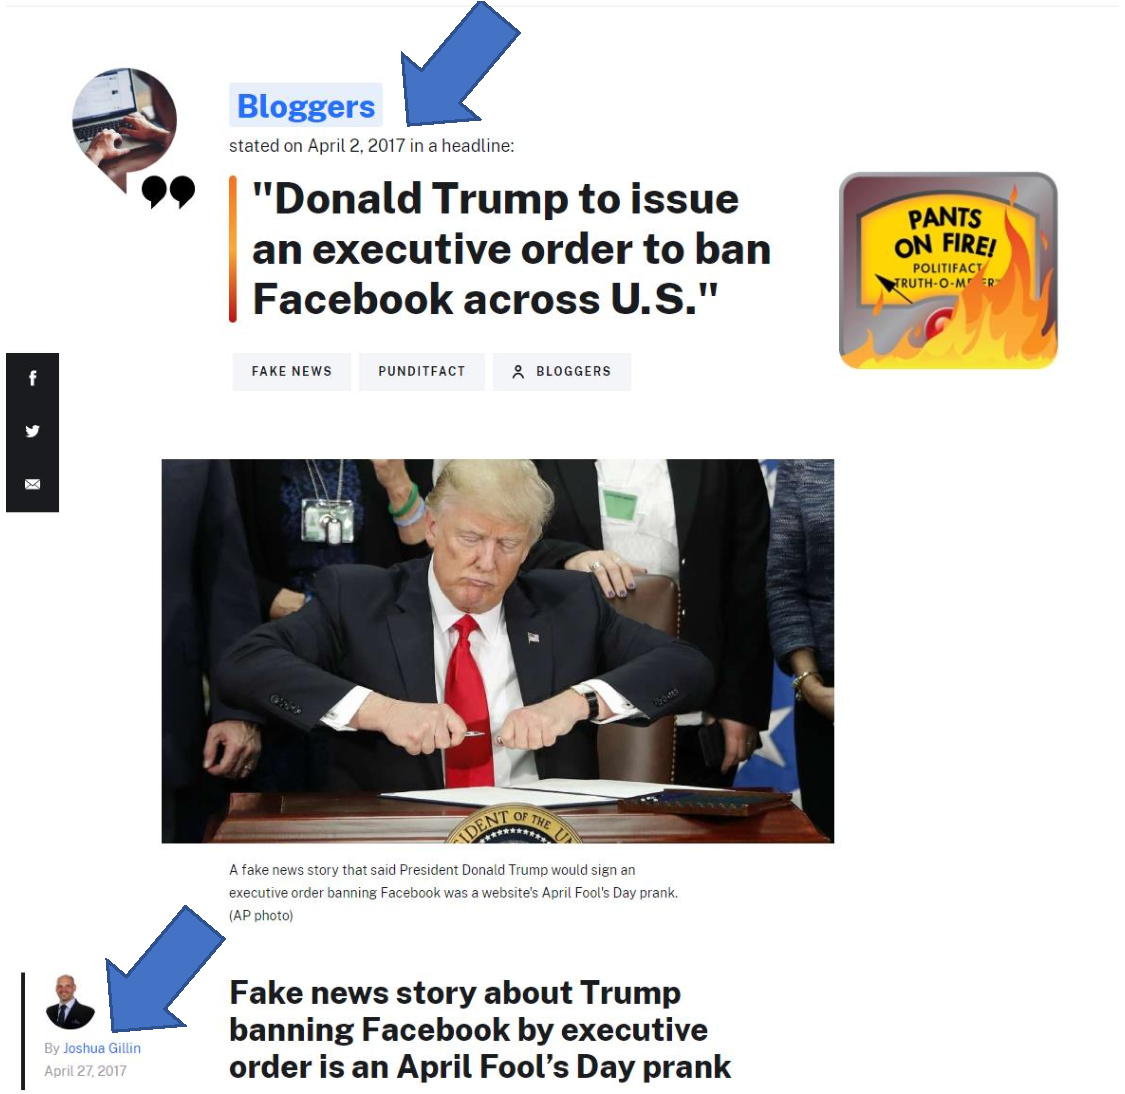
\includegraphics[width=\linewidth]{images/fact-check.pdf}
    \caption{
        北米で行われたファクトチェックの一例。
        % この情報はエイプリルフールで投稿された虚偽情報としている。
        青矢印はフェイクニュース投稿日時とファクトチェック結果投稿日時を示し、両者には25日もの間が開いている。
        }
    \label{fig:example}
\end{figure}

図\ref{fig:example}はファクトチェックの一例である\cite{gillin_2017}。
この実例のように、ファクトチェックは属人的な作業であることに加えて結果公表まで時間がかかるため、
ファクトチェック結果はフェイクニュースそのものに比べて拡散されにくい。
このため、機械学習によってフェイクニュースを自動で検出する研究が行われている。

自動検出にあたって困難な点として、フェイクニュースは人々を騙すために巧妙なつくりをしていることが挙げられる。
このため、単純なルールベース手法による検出は難しい。
検出性能の向上において、記事そのものがもつ情報に加えてソーシャルメディア上での反響を示すソーシャルコンテキスト(リツイート・いいね・リプライなど)
を考慮することが有効であることが先行研究で示されている\cite{Guo:2018:RDH:3269206.3271709}。
しかしながら、ソーシャルコンテキストはユーザの拡散によって生まれるため、この場合も早期の検出には向かない。
これに対して、ニュースに対してソーシャルメディア上で寄せられるコメントで発生しやすい単語を、条件付き変分オートエンコーダ(CVAE)で生成する手法も提案されている\cite{ijcai2018-533}。
この手法は、記事から確率分布とラベルを元に隠し変数を介して生成を行っている。

本研究では、記事と実際に記事に寄せられたコメントから信憑性の学習を行い、記事と限られた数のコメントから別のコメントを予測させた上で真偽を判断するモデルを提案する。
このモデルは、フェイクニュースそのものを生成するモデル\cite{NIPS2019_9106}を拡張する形で実装することでコメントの生成を実現する。
学習では記事と実際に記事に寄せられたコメントを3件、更に真偽ラベルを入力するが、テスト時は記事に加えて実際に寄せられたコメントは2件に制限し、真偽ラベルは入力しない。

我々は提案モデルの検出性能を実際に投稿された情報をもつデータセットによって検証した。

\section{関連研究}
フェイクニュースの自動検出(真偽分類)は、対象をスパム\cite{shen2017discovering}や風評\cite{7023340}、そして虚偽広告\cite{Huang:2017:DFO:3041021.3054233}を含めると新しいトピックではない。
本研究はこれまでの研究\cite{Shu:2017:FND:3137597.3137600,Ruchansky:2017:CHD:3132847.3132877,Wang:2018:EEA:3219819.3219903}に倣い、意図的に作成され、明確に誤りであると確認できるニュースをフェイクニュースと定義する。

\subsection{フェイクニュース検出}
ニュース記事がもつ情報からフェイクニュースを検出する手法は多く提案されている。
文字情報からは、フェイクニュースが独自の書かれ方をする上に感情的な表現を多用することから、文章のスタイル\cite{DBLP:journals/corr/PotthastKRBS17}や感情的表現の頻度\cite{DBLP:journals/corr/abs-1903-01728}を考慮する手法がある。
また、ディープニューラルネットワーク(DNN)によって検出性能が改善された報告\cite{wang-2017-liar,karimi-tang-2019-learning,karimi-etal-2018-multi}も多い。

ソーシャルコンテキストを考慮した手法も多く提案されており、扱うコンテキストの種類によってユーザベース\cite{Castillo:2011:ICT:1963405.1963500,8397048,DBLP:journals/corr/abs-1904-13355}
・投稿ベース\cite{Yang2019UnsupervisedFN,Tacchini2017SomeLI,Jin:2016:NVE:3016100.3016318}
・ネットワークベース\cite{Wu:2018:TFF:3159652.3159677,DBLP:journals/corr/abs-1902-06673}の3種類に分けられる。

ソーシャルコンテキストを利用する手法に共通した問題点として、ソーシャルコンテキストはユーザの拡散によって生まれる情報であるため早期検出に向かない点が挙げられる。
早期検出の実現へ、TCNN-URGという2層の畳み込みニューラルネットワークとCVAEによるユーザレスポンス生成器を組み合わせたモデルも提案されている\cite{ijcai2018-533}。
ニュース記事を畳み込みニューラルネットワークで特徴化してから隠れ変数を算出し、寄せられたコメントとして尤もらしい単語群を生成することで検出性能が改善されることが報告されている。
しかしながら、TCNN-URGはあくまで尤もらしい単語を生成することに限られ、実際のコメントそのものは生成していない。

\subsection{フェイクニュース生成}
\label{subsec:generate}
自然言語生成モデルの1つとして、架空のニュース記事を作成するGroverモデルがある\cite{NIPS2019_9106}。
このモデルはニュース記事データセットから記事をドメイン・著者・投稿日時・見出し・本文の5要素に分け、無作為に要素を削除した記事の残り部分から歯抜け部分を予測させることで訓練している。
興味深い点として、Groverモデルで生成した記事の方が実在の記事よりも読者が信じやすい傾向が報告されていた。
本研究ではこのモデルを拡張することで、より自然なコメントを生成することを目指した。

%\input{chapters/purpose}
\section{提案手法}

先行研究により、自然言語文章生成モデルは言語モデル問題の1つとされており、式\ref{eq:generate}のように
文章$x = \mathrm{w}_1^T = (\mathrm{w}_1, \mathrm{w}_2, ..., \mathrm{w}_T)$
はある単語$\mathrm{w}_t$が生成される前の単語群$ \mathrm{w}_1^{t-1}$による条件付き確率の総積であると定義されている。

\begin{equation}
    \label{eq:generate}
    p(x) = p(\mathrm{w}_1^T) = \prod_{t=1}^{T} p(\mathrm{w}_t|\mathrm{w}_1^{t-1})
\end{equation}

提案モデルによる文章生成の流れは図\ref{fig:method}の通りである。
第\ref{subsec:generate}の通り、ベースとなったGroverモデルは記事を5要素に分けて学習が行われており、
生成及び分類学習において、各要素の始点と終点には開始及び終了トークンが付加されている。
本研究ではこれらの要素を記事本文とそれに寄せられた3件のコメントに置換することで実装する。
ベースとなったモデルに倣い、提案モデルは以下の同時分布として定義する。

\begin{equation}
    \label{eq:joint_distri}
    p(\rm{article}, \rm{comment\_1}, \rm{comment\_2}, \rm{comment\_3})
\end{equation}

コメント生成学習時は、ベースとなったGroverモデルと同様に記事とコメントのセットを2つの集団に分け、無作為に歯抜けにする。
コメントの場合は10\%、記事本文の場合は35\%の確率で歯抜けにしてから一方の集団から学習を行い、もう一方での生成におけるクロスエントロピー誤差を最小化するように訓練される\cite{NIPS2019_9106}。
提案モデルの目的は記事ではなくSNS上で記事に寄せられたユーザの反応を生成することである。

\begin{figure*}[t]
    \centering
    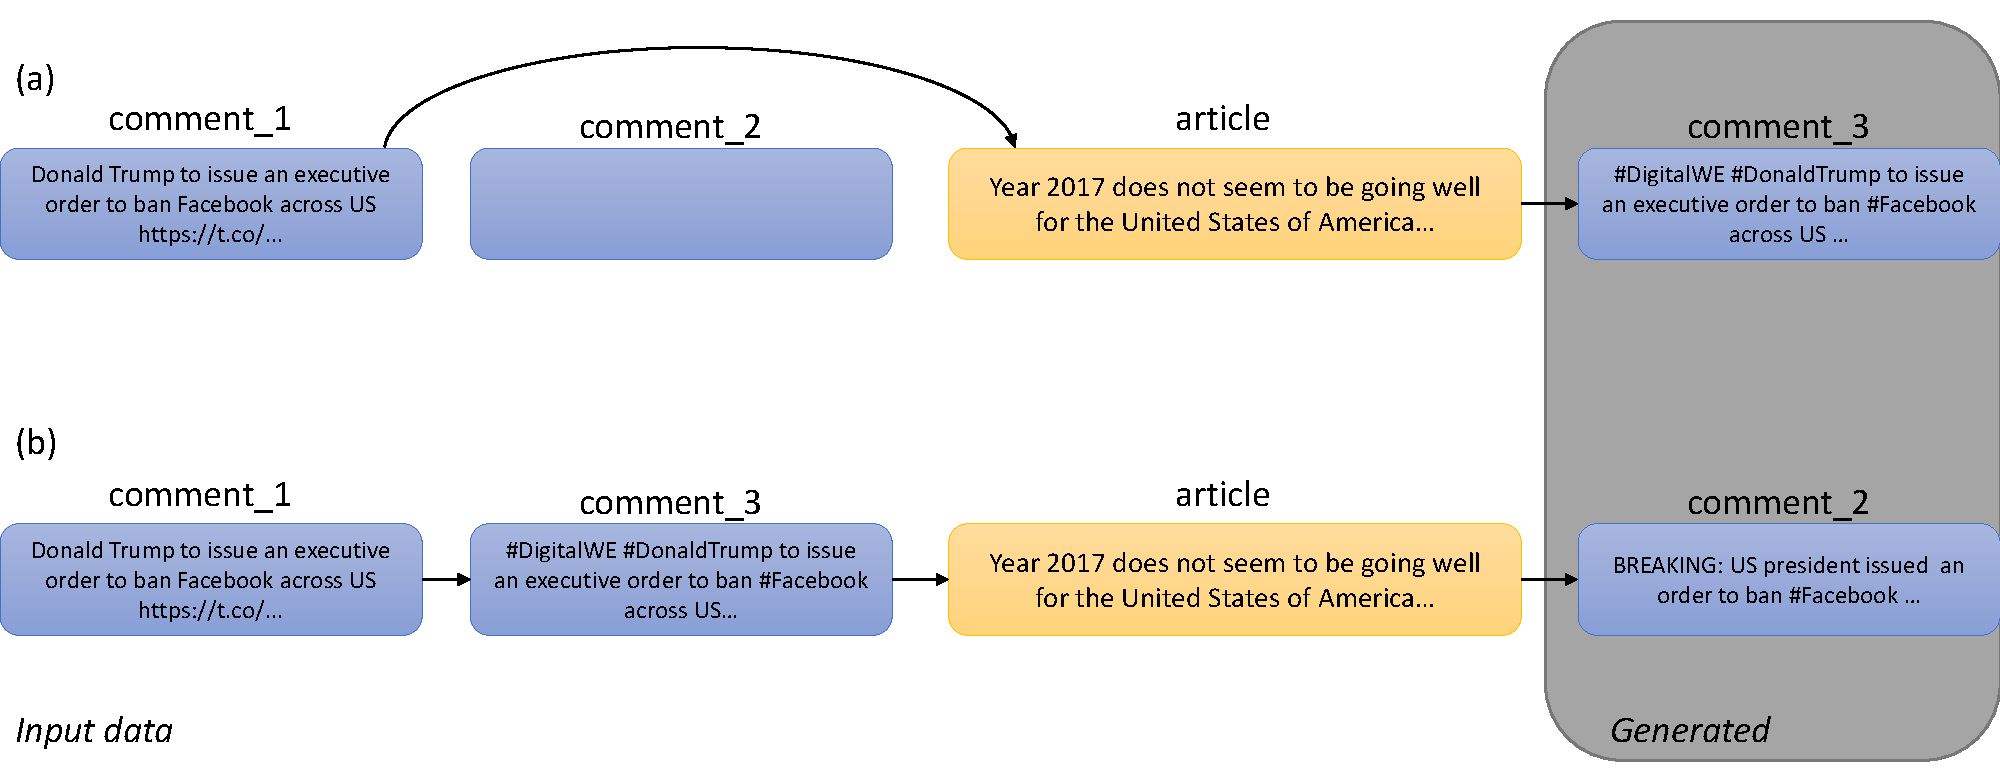
\includegraphics[width=\linewidth,pagebox=cropbox,clip]{images/fig_method.pdf}
    \caption{
        提案モデルのコメント生成例。
        (a)は記事と1件の実際に寄せられたコメントからコメントを生成している。
        (b)は(a)で生成したコメントを含めた状況で更にコメントを生成している。
    }
    \label{fig:method}
\end{figure*}

記事とコメントのセットの末尾にはセットの終端を意味するトークンである\texttt{[CLS]}を追加し、またこのトークンが真偽を分類する際に使われる。
これはGroverモデルがベースとしているGPT-2がとる手法\cite{Radford_GPT2}と同一である。
図は実際の記事とコメントのセットを真偽分類するまでの流れを示している。
まず、記事に寄せられたコメント群から実験に使用するために無作為に3件選出し、コメント生成の学習を行う。
真偽分類する際には、3件の実際に投稿されたコメントから1件削除してから生成されたコメントを追加してから真偽の分類を行う。
また、同時に生成コメントを追加しなかった状況で分類を行った際の結果との比較も行った。

\begin{figure*}[t]
    \centering
    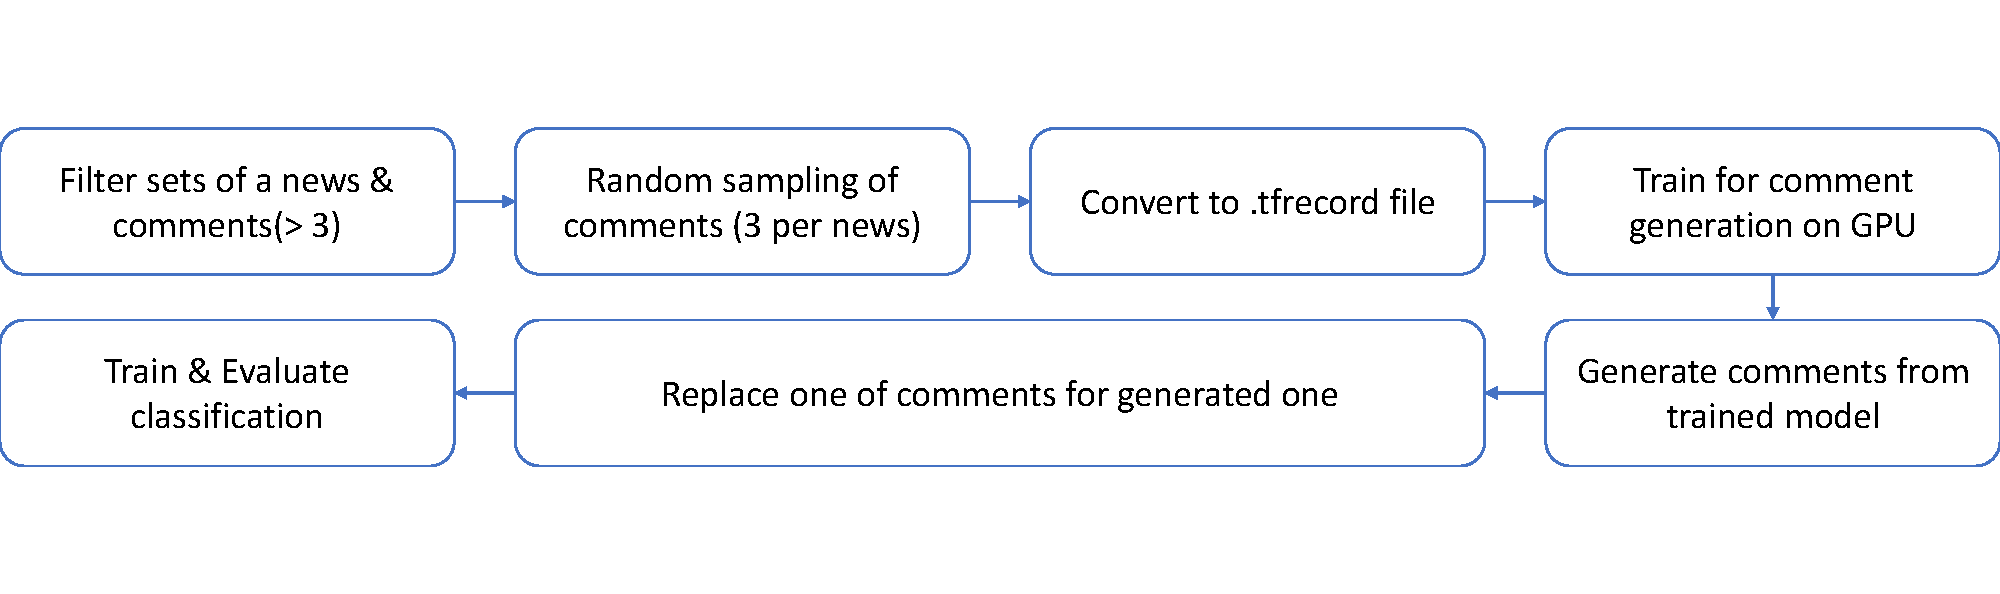
\includegraphics[width=0.8\linewidth,pagebox=cropbox,clip]{images/fig_process.pdf}
    \caption{実験の流れ}
    \label{fig:process}
\end{figure*}

\section{実験}
\subsection{実験環境}
今回の提案モデルの実装や実験の実施は、以下の環境で行った。
\begin{itemize}
    \item TITAN X (Pascal)を搭載したLinuxマシン上のDockerで構築したUbuntu16.04環境で実験を行った。
    \item GitHub上で公開されていたGroverモデルをForkして実装を行った。
    \item モデルサイズはGrover-Baseを採用し、今回実験で使用する語彙サイズに合わせて調整を行った。
\end{itemize}

\subsection{単語生成の傾向}
\label{subsec:trend}
まずはじめに、正しいニュースとフェイクニュースの記事とコメントのセットから生成されたコメントの傾向を調べた。
いずれもニュース記事とコメントのセットはFakeNewsNetデータセット\cite{Shu2018FakeNewsNetAD}から取得した。
このデータセットは北米で英文記事を対象にファクトチェックを行う団体であるPolitiFact(政治ニュース中心)とGossipCop(芸能ニュース中心)の判断結果を元に正しいニュースとフェイクニュースのラベルが付けられている。
我々はまず実験手法に合わせるために記事に対して最低3件以上コメントが寄せられているセットに対して無作為に3件選出した。
また、PolitiFactから真偽で各200セットを用意して学習を行った。
実際に生成されたコメントに対して、すべてアルファベットを小文字にした上で単語ごとの出現回数と出現確率を算出した。
また、算出するにあたって記号(クォーテーションやピリオド、コンマなど)やURLの削除を行ったほか、``a''や``is''といったストップワードはNLTK\cite{bird-loper-2004-nltk}が提供するメソッドを使用して除外した。
なお、コメントの収集元がTwitterであることから、Twitter独自の用法をもつ記号(ハッシュタグ\#やメンション@)、またコロンは例外として除外しなかった。
以上の処理を行った結果、以下の特徴が得られた。

\begin{itemize}
    \item 真偽問わず最も頻度が高い単語は``via''であり、真偽全体の単語のうち約1.5\%を占めた。
    \item それに続いて``trump''と``obama''が続いたが、いずれも割合は1\%を下回った。
\end{itemize}

また、真偽における傾向差として以下の違いが見られた。

\begin{itemize}
    \item ``via''は真偽単独で見てもそれぞれで最も高い頻度で生成されていた。
    \item フェイクにおける``via''の生成頻度は正しい場合に比べて約2倍であり、その差は約0.9ポイントとフェイク頻出上位10単語中最多だった。
    \item ``breaking:''という単語が``via''に次いで2番目に頻度の差が高い単語であり、その差は0.7ポイントだった。
\end{itemize}

\subsection{検出における生成コメントの影響}
生成コメントの有無によって真偽分類の結果に影響が出るか調べた。
ベースラインとして2つの入力データを用意した。
1つは生成されたコメントを入力せず、記事と実際に投稿された2件のコメントから分類させた場合、
もう1つは実際に投稿されたコメントも入力せず、記事のみから分類させた場合であった。
この実験では、PolitiFactでは十分な量の学習を行うにはセット数が少なかったため、GossipCopから真偽で各2000セットを用意して行った。
実験結果は表\ref{tbl:classify_results}の通りである。
提案モデルは再現率において全体ベストとなったものの、適合率においては生成モデルを使わない方が優秀であることが読み取れる。
また、生成されたコメントには共通して文法面にさらなる改善の必要性が残された。

\begin{table}[!t]
    \renewcommand{\arraystretch}{1.3}
    \caption{分類成績}
    \label{tbl:classify_results}
    \centering
    \begin{tabular}{lccc}
        \hline
        入力データ           & 適合率 & 再現率 & F値 \\ \hline
        記事本文のみ         & 0.647     & 0.615  & 0.631    \\
        + 実在コメント2件  & \textbf{0.682}     & 0.750  & \textbf{0.714}    \\
        + 生成コメント1件 & 0.590     & \textbf{0.790}  & 0.675    \\ \hline
    \end{tabular}
\end{table}

\section{考察}
\subsection{コメント生成}
コメント生成の傾向から、提案モデルは入力されたニュース記事が扱うトピックの学習に成功したように見える。
生成されたコメントの多くが政治的内容を含むものが多かった理由として、データセットが扱う内容の影響を受けたことが考えられる。

生成コメントの中で興味深い単語は``breaking:''である。
この単語はフェイクニュースに寄せられたコメントとして生成されていた。
本研究と同じくコメントとして尤もらしい単語を生成するTCNN-URG\cite{ijcai2018-533}でも、
フェイクを示すシグナルとして``!''や``?''、そして``false''が報告されていたが、``breaking:''は報告されていなかった。
よって、この``breaking:''もフェイクニュースを示す重要なシグナルである可能性がある。

生成されたコメントは軒並み文法面に改善点が残されているが、これはデータセットの規模不足が原因として考えられる。
Groverモデルは120GBにも及ぶニュースデータセットから訓練されていた\cite{NIPS2019_9106}ことも考慮すると、
改善のためにはさらなる追加データを収集する必要がある可能性が示されている。

\subsection{真偽分類}
表\ref{tbl:classify_results}を見るに、提案モデルは再現率は優秀だったが適合率に大きな課題を残した。
これは提案モデルがソーシャルコンテキストが制限されている状況でも、制限されたまま真偽分類を行うより多くのフェイクニュースの検出ができることを意味する。

この傾向はファクトチェックが必要なニュースを探す際に役立つことを示唆している。
ただし適合率が低いため他のモデルより多く正しいニュースをフェイクニュースとして誤って検出するため、改善が求められている。
今後は、より多くのデータセットを用いた場合に傾向が変化するか調べる必要があるとみられる。

\section{結論}
本研究では、フェイクニュースの早期発見における問題点の解決を試みた。
我々は、ユーザのコメントはニュース記事を評価する際で重要な情報をもたらすものの、
ニュース拡散の初期段階ではコメントが少ない点に着目する。
そこで、Groverモデルを拡張したニューラルネットワークモデルを作成し、分類に有用なコメントを生成することを提案する。
提案モデルのコメント生成による早期発見性能を評価するために、実際のニュースとそれに寄せられたコメントを対象に実験を行った。
その結果、コメントを生成するプロセスが、ファクトチェックによって真偽を判定する際に役立つ可能性が示唆されている。

%謝辞
%\section*{謝辞}
%\addcontentsline{toc}{section}{謝辞}
\begin{acknowledgment}
    本研究はJSPS科研費 JP17H04705,JP18H03229,JP18H03340,JP18K19835,JP19H04113,JP19K12107の助成を受けたものです。
    本研究を遂行するにあたり、研究の機会と議論・研鑽の場を提供して頂き、御指導頂いた早稲田大学 本位田真一教授、鄭顕志准教授をはじめ、活発な議論と貴重な御意見を頂いた研究グループの皆様に感謝致します。
\end{acknowledgment}


%また,研究の機会と議論・研鑽の場を提供して頂き,ご指導頂いた国立情報学研究所/東京大学の本位田真一教授をはじめ活発な議論と貴重なご意見を頂いた研究グループの皆様,大須賀・田原研究室の皆様に感謝の意を表します.さらに,本研究を行う上で必要な楽天公開データの提供に協力してくださいました国立情報学研究所,楽天株式会社の関係者の皆様に感謝の意を表します.

%\section*{研究業績}
%\addcontentsline{toc}{section}{研究業績}

%\subsection*{国際会議}
%\begin{achievement}
%\item \underline{\textbf{Minato Sato}}, Ryohei Orihara, Sei Yuichi, Yasuyuki Tahara and Akihiko Ohsuga: Japanese Text Classification by Character-Level Deep ConvNets and Transfer Learning, The 9th International Coneference on Agents and Artificial Intelligence (ICAART2017), Feb 2017. (accepted as a Full Paper)
%\end{achievement}

%\subsection*{査読付き国内シンポジウム・ワークショップ}
%\begin{achievement}
%\item \underline{\textbf{佐藤挙斗}},折原良平,清雄一,田原康之,大須賀昭彦: 文字レベル深層学習による日本語テキストの分類と転移学習,合同エージェントワークショップ&シンポジウム2016 (JAWS2016),pp.199-206,2016年9月. (ショート発表) \textcolor{red}{{\bf 優秀発表賞}}
%\end{achievement}

%\subsection*{研究会}
%\begin{achievement}
%\item \underline{\textbf{佐藤挙斗}},折原良平,清雄一,田原康之,大須賀昭彦: 文字レベル深層学習の日本語データセットへの応用,第184回 情報処理学会 知能システム研究会 (SIG-ICS) ,2016年8月.
%\item \underline{\textbf{佐藤挙斗}},折原良平,清雄一,田原康之,大須賀昭彦: 文字レベル深層学習によるテキスト分類と転移学習,人工知能学会 第102回人工知能基本問題研究会(SIG-FPAI),2016年12月. 
%\end{achievement}

%付録
%\appendix
%A.1
\section{実験環境}
\label{app:settings}
\begin{itemize}
    \item TITAN X (Pascal)を搭載したLinuxマシン上のDockerで構築したUbuntu16.04環境で実験を行った。
    \item GitHub上で公開されていたGroverモデルをForkして実装を行った。
    \item モデルサイズはGrover-Baseを採用し、今回実験で使用する語彙サイズに合わせて調整を行った。
\end{itemize}

\bibliographystyle{junsrt}
\bibliography{reference}
\end{document}